% Options for packages loaded elsewhere
\PassOptionsToPackage{unicode}{hyperref}
\PassOptionsToPackage{hyphens}{url}
\PassOptionsToPackage{dvipsnames,svgnames,x11names}{xcolor}
%
\documentclass[
  11pt,
]{article}
\usepackage{amsmath,amssymb}
\usepackage{iftex}
\ifPDFTeX
  \usepackage[T1]{fontenc}
  \usepackage[utf8]{inputenc}
  \usepackage{textcomp} % provide euro and other symbols
\else % if luatex or xetex
  \usepackage{unicode-math} % this also loads fontspec
  \defaultfontfeatures{Scale=MatchLowercase}
  \defaultfontfeatures[\rmfamily]{Ligatures=TeX,Scale=1}
\fi
\usepackage{lmodern}
\ifPDFTeX\else
  % xetex/luatex font selection
  \setmainfont[]{Latin Modern Roman}
  \setsansfont[]{Latin Modern Sans}
  \setmonofont[Scale=0.82]{DejaVu Sans Mono}
\fi
% Use upquote if available, for straight quotes in verbatim environments
\IfFileExists{upquote.sty}{\usepackage{upquote}}{}
\IfFileExists{microtype.sty}{% use microtype if available
  \usepackage[]{microtype}
  \UseMicrotypeSet[protrusion]{basicmath} % disable protrusion for tt fonts
}{}
\makeatletter
\@ifundefined{KOMAClassName}{% if non-KOMA class
  \IfFileExists{parskip.sty}{%
    \usepackage{parskip}
  }{% else
    \setlength{\parindent}{0pt}
    \setlength{\parskip}{6pt plus 2pt minus 1pt}}
}{% if KOMA class
  \KOMAoptions{parskip=half}}
\makeatother
\usepackage{xcolor}
\usepackage[margin=25mm]{geometry}
\usepackage{longtable,booktabs,array}
\usepackage{calc} % for calculating minipage widths
% Correct order of tables after \paragraph or \subparagraph
\usepackage{etoolbox}
\makeatletter
\patchcmd\longtable{\par}{\if@noskipsec\mbox{}\fi\par}{}{}
\makeatother
% Allow footnotes in longtable head/foot
\IfFileExists{footnotehyper.sty}{\usepackage{footnotehyper}}{\usepackage{footnote}}
\makesavenoteenv{longtable}
\usepackage{graphicx}
\makeatletter
\def\maxwidth{\ifdim\Gin@nat@width>\linewidth\linewidth\else\Gin@nat@width\fi}
\def\maxheight{\ifdim\Gin@nat@height>\textheight\textheight\else\Gin@nat@height\fi}
\makeatother
% Scale images if necessary, so that they will not overflow the page
% margins by default, and it is still possible to overwrite the defaults
% using explicit options in \includegraphics[width, height, ...]{}
\setkeys{Gin}{width=\maxwidth,height=\maxheight,keepaspectratio}
% Set default figure placement to htbp
\makeatletter
\def\fps@figure{htbp}
\makeatother
\setlength{\emergencystretch}{3em} % prevent overfull lines
\providecommand{\tightlist}{%
  \setlength{\itemsep}{0pt}\setlength{\parskip}{0pt}}
\setcounter{secnumdepth}{-\maxdimen} % remove section numbering
\ifLuaTeX
\usepackage[bidi=basic]{babel}
\else
\usepackage[bidi=default]{babel}
\fi
\babelprovide[main,import]{english}
\ifPDFTeX
\else
\babelfont{rm}[]{Latin Modern Roman}
\fi
% get rid of language-specific shorthands (see #6817):
\let\LanguageShortHands\languageshorthands
\def\languageshorthands#1{}
\usepackage{microtype}
\usepackage{float}
\usepackage{fancyhdr}
\usepackage{needspace}
\floatplacement{figure}{H}
\pagestyle{fancy}
\fancyhf{}
\fancyhead[L]{\small\sffamily Shared temporal scale across bodily judgments}
\fancyhead[R]{\small\sffamily CTD v0.1.0}
\fancyfoot[C]{\small\thepage}
\setlength{\headheight}{14pt}
\renewcommand{\headrulewidth}{0.3pt}
\setlength{\emergencystretch}{3em}
\widowpenalty=10000
\clubpenalty=10000
\makeatletter
\let\ctdoldsection\section
\renewcommand{\section}{\Needspace{8\baselineskip}\ctdoldsection}
\let\ctdoldsubsection\subsection
\renewcommand{\subsection}{\Needspace{6\baselineskip}\ctdoldsubsection}
\makeatother
\ifLuaTeX
  \usepackage{selnolig}  % disable illegal ligatures
\fi
\IfFileExists{bookmark.sty}{\usepackage{bookmark}}{\usepackage{hyperref}}
\IfFileExists{xurl.sty}{\usepackage{xurl}}{} % add URL line breaks if available
\urlstyle{same}
\hypersetup{
  pdftitle={Testing a Shared Temporal Scale Across Bodily Judgments},
  pdfauthor={Hongju Liu},
  pdflang={en},
  colorlinks=true,
  linkcolor={NavyBlue},
  filecolor={Maroon},
  citecolor={Blue},
  urlcolor={NavyBlue},
  pdfcreator={LaTeX via pandoc}}

\title{Testing a Shared Temporal Scale Across Bodily Judgments}
\usepackage{etoolbox}
\makeatletter
\providecommand{\subtitle}[1]{% add subtitle to \maketitle
  \apptocmd{\@title}{\par {\large #1 \par}}{}{}
}
\makeatother
\subtitle{Exact cross-task constraints and a secondary analysis of
parietal stimulation}
\author{Hongju Liu}
\date{10 October 2026 · CTD-PAPER-v0.1.0}

\begin{document}
\maketitle

\textbf{Affiliation:} Independent researcher, Shenzhen, China.

\textbf{Status:} Complete working manuscript for scientific review; not
externally peer reviewed. This is a retrospective secondary analysis of
public human data and a mathematical methods application. No new
participants, neural interventions, or hardware experiments were
conducted. This edition has no assigned DOI. The source experiment, its
original findings, and its released fitted parameters belong to D'Angelo
and colleagues {[}1{]}.

\hypertarget{abstract}{%
\section{Abstract}\label{abstract}}

A physical intervention can affect two bodily judgments without
demonstrating that their changes are proportional expressions of one
shared temporal process. Conversely, failure of proportionality need not
imply separate processes when task-specific measurement relations are
nonlinear. We distinguish these claims using two explicit models of
positive psychometric widths: a shared multiplicative scale and a shared
scalar with stable increasing task maps. For two tasks, the exact
smallest uniform log adjustment required by the multiplicative model is
one quarter of the range of the between-task log-width differences. The
corresponding distance to a common nondecreasing order is obtained by a
finite isotonic construction. These are applications of established
measurement and approximation principles, with complete proofs and
computational checks. We apply them to the 30-participant
parietal-stimulation experiment of D'Angelo et al.~(2026), retaining the
original authors' prior stimulation, covariance, and Bayesian-model
results as inherited evidence. In 180 released width estimates, the mean
difference between the tasks' 8-Hz/13-Hz log gains is −0.0146 (95\% CI
−0.0933 to 0.0642; paired \(t_{29}=-0.378\), \(p=.708\)). The median
descriptive adjustment budget for individual proportionality is 4.20\%;
25 of 30 estimated profiles have matching condition order. These
point-estimate diagnostics are not individual violation tests. A
separately specified binomial response model tests all 60 within-person
restrictions in the 1,260 count cells; its likelihood-ratio statistic is
73.813, with conditional parametric-bootstrap \(p=.105\). Its
uncertainty remains separate from the released widths. The results do
not identify a neural mediator, establish an experiential scale, or
select a global consciousness theory. They supply a reproducible test of
explicit model-and-measurement conjunctions and identify the additional
calibration needed for a discriminating experiment.

\textbf{Keywords:} body ownership; simultaneity judgment; causal
intervention; psychometric width; state-trace analysis; measurement
invariance; UCT.

\hypertarget{from-source-identification-to-a-discriminating-prediction}{%
\section{1. From source identification to a discriminating
prediction}\label{from-source-identification-to-a-discriminating-prediction}}

Suppose two systems behave alike and predict the same consequences.
Their successful outputs do not determine which sources their internal
consumers use. \emph{Matched Behavior and Source Use} formalized this
problem in finite sensorimotor models, giving exact intervention
requirements and counterexamples to common identification shortcuts
{[}2{]}. Its question was organizational: which route is used, under
which assumptions? A further question concerns explanation: once an
intervention has been performed, what result could distinguish competing
accounts of the relevant bodily judgment?

That second question requires more than a change in a measured outcome.
An intervention on a shared brain region may influence ownership
judgments and simultaneity judgments through a common latent variable,
several task-specific paths, a change in decision criteria, or a
combination. Even if a shared variable is a good explanation, the tasks
may express it on different nonlinear scales. A numerical interaction
can then be produced or removed by the measurement relation. This
problem has a long history in measurement theory, interaction
interpretation, and state-trace analysis {[}3--9,17{]}. We do not claim
to introduce it.

We examine a specific additional restriction in a real intervention
dataset. D'Angelo et al.~studied parietal alpha frequency, body
ownership, and visuotactile simultaneity {[}1{]}. Their Experiment 3
manipulated stimulation condition within participants and measured both
judgments. The original study already reported effects on both tasks,
individual cross-task correlations of intervention effects, and a
comparison of Bayesian causal-inference models with changing sensory
uncertainty or changing common-cause priors. The present analysis asks a
stricter question: \textbf{can each participant's positive task widths
be represented by one stimulation-dependent multiplicative factor and a
task factor that remains fixed across stimulation?}

The proposed restriction is not asserted to be a necessary prediction of
the original study's Bayesian model. A shared uncertainty parameter can
have different nonlinear consequences for two response functions and
their fitted widths. Nor does the restriction follow from Unified
Consciousness Theory (UCT), whose structural correspondence axiom does
not supply an empirical task-to-experience measurement law {[}10,11{]}.
It is a deliberately added, falsifiable bridge.

The contribution is consequently narrow and inspectable. We formulate
the proportional restriction and a weaker ordinal alternative; derive
their exact adjustment budgets; retrospectively test the new constraint
on released human data; and separate the resulting evidence from claims
about neural mediation or experience. The application also illustrates
why the existence of a usable dataset does not remove the need to audit
the fitted estimator, the unit of analysis, and the theoretical
interpretation of the endpoint.

\hypertarget{models-and-targets}{%
\section{2. Models and targets}\label{models-and-targets}}

\hypertarget{the-measured-object}{%
\subsection{2.1 The measured object}\label{the-measured-object}}

Let \(i\) index a participant, \(t\in\{O,S\}\) the ownership and
simultaneity tasks, and \(f\) one of the stimulation conditions. Write
\(W_{itf}>0\) for the width parameter of a specified task-response
function. An estimate is \(\widehat W_{itf}\). A psychometric width, a
sensory-noise parameter in a generative model, a neuronal integration
time, a report of ownership, and a selected experiential property are
distinct objects.

This separation matters empirically. Yarrow et al.~manipulated judgment
strategy and showed that the fitted window of subjective synchrony can
change with strategy {[}7{]}. Width is therefore not automatically a
direct sensory or neural clock reading. In this paper, \emph{shared
temporal scale} names a mathematical model of positive task widths.
Physical and phenomenal interpretations require additional evidence.

The two models below are applied separately within each participant. The
task maps remain fixed across the specified stimulation conditions; that
invariance is a substantive assumption, not a consequence of the data
table.

\hypertarget{a-proportional-bridge-and-its-ordinal-relaxation}{%
\subsection{2.2 A proportional bridge and its ordinal
relaxation}\label{a-proportional-bridge-and-its-ordinal-relaxation}}

The strict multiplicative bridge is

\[
\mathcal M_\times:\qquad W_{itf}=c_{it}\tau_{if},
\qquad c_{it}>0,\quad \tau_{if}>0.
\]

The task factor \(c_{it}\) does not depend on stimulation. Under this
bridge, changing stimulation changes both task widths by the same ratio
for the same person. Multiplicative task calibration cancels in a
within-task ratio. An arbitrary additive offset on the original width
scale does not cancel.

A weaker model allows nonlinear task maps:

\[
\mathcal M_\uparrow:\qquad W_{itf}=h_{it}(\tau_{if}),
\]

where the maps are strictly increasing and fixed across conditions. Its
finite-data closure, \(\overline{\mathcal M}_\uparrow\), permits
nondecreasing maps, including task-specific plateaus. Every proportional
bridge is a strict monotone bridge, but the converse is false. These are
instances of established common-latent-order and state-trace ideas
{[}3--6{]}.

The models make different observable demands. The proportional model
requires equal ratios. The strict ordinal model requires the same
ordering and matching ties. Allowing condition-dependent task maps
without restriction removes both demands. Calling a variable ``shared''
then supplies little testable content.

Neither a fitted proportional representation nor an ordinal
representation establishes that the physical system has only one cause.
These models constrain a selected view of the outcomes. Multiple
physical implementations can induce the same table, as the prior
source-consumer analysis also illustrates {[}2{]}.

\hypertarget{exact-model-boundaries}{%
\section{3. Exact model boundaries}\label{exact-model-boundaries}}

We suppress \(i\) in this section. Put \(\ell_{tf}=\log W_{tf}\) and
\(d_f=\ell_{Of}-\ell_{Sf}\).

\hypertarget{characterization-and-a-sharp-proportional-adjustment}{%
\subsection{3.1 Characterization and a sharp proportional
adjustment}\label{characterization-and-a-sharp-proportional-adjustment}}

\textbf{Proposition 1.} The following conditions are equivalent:

\[
W_{tf}=c_t\tau_f;\qquad
\ell_{tf}=a_t+b_f;\qquad
d_f=d_g\ \text{for all }f,g;
\]

\[
W_{Of}W_{Sg}=W_{Og}W_{Sf}\ \text{for all }f,g.
\]

\textbf{Proof.} Taking logarithms gives an additive model, and
subtracting its rows gives the constant \(a_O-a_S\). Conversely, if the
row difference is the constant \(d\), choose \(a_O=d\), \(a_S=0\), and
\(b_f=\ell_{Sf}\). Exponentiating recovers the positive multiplicative
model. The cross-product equalities are the exponentiated row-difference
equalities. \(\square\)

This is the familiar positive rank-one condition and its log-additive
form. With two tasks and three conditions there are two independent
restrictions per participant. A single 8-Hz/13-Hz contrast is only one
necessary restriction.

\textbf{Theorem 1.} The minimum uniform change on the log scale needed
to fit the proportional model is

\[
\varepsilon_\times^*
=\inf_{a,b}\max_{t,f}|\ell_{tf}-a_t-b_f|
=\frac{\max_f d_f-\min_f d_f}{4}.
\]

\textbf{Proof.} If \(\ell_{tf}=a_t+b_f+e_{tf}\) and
\(|e_{tf}|\leq\varepsilon\), then \(d_f=(a_O-a_S)+(e_{Of}-e_{Sf})\).
Each difference lies within \(2\varepsilon\) of the same constant, so
its total range is at most \(4\varepsilon\). This proves necessity. For
sufficiency, let

\[
c=\frac{\max_f d_f+\min_f d_f}{2},\quad
a_O=c/2,\quad a_S=-c/2,\quad
b_f=(\ell_{Of}+\ell_{Sf})/2.
\]

The two residuals in condition \(f\) are \((d_f-c)/2\) and its negative.
Their largest magnitude is exactly one quarter of the range of \(d_f\).
\(\square\)

This elementary Chebyshev-approximation result gives an interpretable
diagnostic. At the optimal budget, every corrected width can be kept
inside

\[
e^{-\varepsilon_\times^*}
\leq W^*_{tf}/W_{tf}
\leq e^{\varepsilon_\times^*}.
\]

The reported percentage \(100(e^{\varepsilon_\times^*}-1)\) denotes an
upper multiplicative allowance; the corresponding downward allowance is
\(100(1-e^{-\varepsilon_\times^*})\). It does not mean that every cell
must move by that percentage. It is the smallest common maximum
allowance that makes some correction feasible.

For estimated widths, this is a distance of point estimates. It is not a
measurement-error estimate, a confidence interval, or proof of an
additional neural pathway. Sampling error, unstable response criteria,
model misspecification, and task-specific effects can all contribute to
the same distance.

\hypertarget{what-defensible-error-bounds-would-add}{%
\subsection{3.2 What defensible error bounds would
add}\label{what-defensible-error-bounds-would-add}}

Suppose the true log widths belong to a simultaneous rectangular set
\(\ell_{tf}\in[L_{tf},U_{tf}]\). Define \(D_f^-=L_{Of}-U_{Sf}\) and
\(D_f^+=U_{Of}-L_{Sf}\). The smallest proportional distance attained by
any log-width table in that uncertainty rectangle is

\[
\varepsilon_{\times,\mathrm{box}}^*
=\frac{[\max_f D_f^- -\min_f D_f^+]_+}{4}.
\]

\textbf{Proof.} Each task difference can be selected independently
inside \([D_f^-,D_f^+]\). If all these intervals intersect, the selected
differences can be equal. Otherwise every selection must span the gap
between the largest lower endpoint and smallest upper endpoint. Choosing
values within that gap and their respective intervals attains the
minimum range. Theorem 1 completes the result. \(\square\)

This is a deterministic statement. Separate marginal 95\% intervals are
not automatically a simultaneous 95\% rectangle. We do not use this
formula to invent uncertainty for the released fitted widths. It
specifies exactly what independently defensible uncertainty would be
needed to turn a descriptive incompatibility into a robust one.

\hypertarget{the-ordinal-model-and-its-sharp-distance}{%
\subsection{3.3 The ordinal model and its sharp
distance}\label{the-ordinal-model-and-its-sharp-distance}}

\textbf{Proposition 2.} Fixed strictly increasing task maps represent
the width table if and only if

\[
\operatorname{sign}(W_{Of}-W_{Og})
=\operatorname{sign}(W_{Sf}-W_{Sg})
\quad\text{for all }f,g.
\]

\textbf{Proof.} Strictly increasing maps preserve each ordering and each
tie of their common input. Conversely, partition the conditions into
their common tied classes, assign increasing latent values to the
classes, and interpolate each task's corresponding values with a
strictly increasing function on the relevant latent span. \(\square\)

To measure distance to the nondecreasing closure, let \(\pi\) be a
permutation of the \(F\) conditions. Define

\[
\varepsilon(\pi)
=\frac12\max_{t,\,j<k}
[\ell_{t,\pi_j}-\ell_{t,\pi_k}]_+.
\]

\textbf{Theorem 2.} The smallest uniform log correction admitting a
common nondecreasing condition order is

\[
\varepsilon_\uparrow^*=\min_\pi\varepsilon(\pi).
\]

For three conditions only six orders need consideration.

\textbf{Proof.} For a fixed order, any corrected nondecreasing sequence
within \(\varepsilon\) of the observed row can remove an inversion of at
most \(2\varepsilon\). This gives the lower bound. Conversely, if all
inversions are at most \(2\varepsilon\), set

\[
m_{t,\pi_k}=\max_{j\leq k}(\ell_{t,\pi_j}-\varepsilon).
\]

The sequence is nondecreasing, at least \(\ell_{t,\pi_k}-\varepsilon\),
and at most \(\ell_{t,\pi_k}+\varepsilon\). It therefore attains a
feasible correction. Minimizing over common orders proves the result.
\(\square\)

This is standard \(L_\infty\) isotonic reasoning applied to a shared
ordering {[}5,6{]}. For exactly two tasks, an independent equivalent
form is half the largest, across oppositely ordered condition pairs, of
the smaller absolute task gap. The supplement proves and checks that
equivalence; the analysis uses the transparent six-order enumeration.

The closure qualification matters. Log-width rows \((0,0,1)\) and
\((0,1,2)\) have zero distance to a common nondecreasing order but
incompatible exact ties for strictly increasing maps. Strict
common-order matrices can approach them arbitrarily closely. Thus zero
distance to the closure is not always exact strict representability.

Because the proportional class is contained in the ordinal class,

\[
0\leq\varepsilon_\uparrow^*\leq\varepsilon_\times^*.
\]

An ordinal-compatible table can fail proportionality. A reliably
positive ordinal distance would require relaxing at least one of the
stable increasing-map, common-scalar, endpoint-model, or measurement
assumptions. It would not by itself identify which assumption failed.

\hypertarget{four-instructive-counterexamples}{%
\subsection{3.4 Four instructive
counterexamples}\label{four-instructive-counterexamples}}

\textbf{Nonlinearity without a second scalar.} Let \(\tau=(1,2,4)\),
\(W_O=\tau\), and \(W_S=\tau^2\). The two tasks have the same strict
order and one scalar input, but unequal proportional gains. Here
\(\varepsilon_\times^*=\frac12\log2\) and \(\varepsilon_\uparrow^*=0\).

\textbf{An ordinal conflict.} For log rows \((0,1,2)\) and \((0,2,1)\),
the last two conditions reverse. Both distances are \(1/2\). Moving both
last values in both rows to \(3/2\) attains the boundary. A smaller
uniform correction cannot remove the reversal.

\textbf{Unrestricted task drift.} Take \(\tau_f=1\) in every condition
and let \(h_{tf}(z)=W_{tf}z\). Every positive table is reproduced, with
an increasing map in each condition. The shared-variable statement has
lost its cross-condition restriction because the task map can change
freely.

\textbf{Cancellation across people.} Participant A has log rows
\((0,1,0)\) and \((0,0,0)\); participant B has the rows interchanged.
Both have proportional distance \(1/4\), while the mean log rows are
identical. A zero population mean interaction cannot establish
individual proportionality. Conversely, noise creates positive
individual distances even under an exact true model.

The supplied finite verification checks all 729 two-by-three log
matrices with entries in \(\{-1,0,1\}\). Independent feasible
constructions and 4,392,225 comparisons against common-order half-grid
corrections agree with the formulas. These computations verify
implementation and examples; the proofs establish the general
finite-condition claims.

\hypertarget{data-and-analysis}{%
\section{4. Data and analysis}\label{data-and-analysis}}

\hypertarget{source-and-provenance}{%
\subsection{4.1 Source and provenance}\label{source-and-provenance}}

We use public Experiment 3 data from D'Angelo et al.~{[}1{]}: 30
analyzed participants, two tasks, three stimulation conditions (8 Hz,
sham, 13 Hz), seven stimulus-onset asynchronies, and ten binary
judgments in each participant-by-task-by-condition-by-asynchrony cell.
The public workbook contains 1,260 yes-count cells, representing 12,600
judgments, and 180 fitted widths. These are repeated observations from
30 people, not 12,600 independent participants.

The seven asynchronies are −400, −200, −100, 0, 100, 200, and 400 ms.
Participant row order and the published task/condition column mapping
were retained; trial chronology and block identifiers were not
available. The source sample was selected for susceptibility to the
ownership illusion (30 analyzed from 37 recruited), limiting population
generalization. We use the original authors' pseudorandomized
stimulation order and reported procedural controls as source-study
assumptions; this reanalysis does not independently validate stimulation
targeting or identify a neural mediator.

The OSF file \texttt{Experiment\_3.xlsx} was downloaded from the
authors' linked project. Its SHA-256 is recorded in the reproducibility
manifest. The final three fitted-width headers duplicate the ownership
labels. Their values were independently matched, cell for cell, to the
publisher's Figure 6c source-data sheet, while the first three matched
Figure 6a. The count blocks likewise exactly matched Figures 6b and 6d.
We preserve original bytes and document the task mapping explicitly,
rather than changing the source workbook.

The original authors already reported cross-task correlations of
intervention effects, approximately \(r=.728\) for sham-minus-8-Hz
changes and \(r=.547\) for 13-Hz-minus-sham changes. Our code reproduces
those values as a mapping check. Their correlations and Bayesian
sensory-uncertainty comparison are not new findings of this paper.
Correlated absolute changes do not entail equal proportional changes.

\hypertarget{retrospective-plan-and-released-width-estimand}{%
\subsection{4.2 Retrospective plan and released-width
estimand}\label{retrospective-plan-and-released-width-estimand}}

This is a retrospective analysis. The source article and some aggregate
findings were inspected before selecting the question. A local analysis
plan was saved before computing the new inferential contrasts; it is not
a prospective preregistration. The model-distance diagnostics and
tolerance sensitivity analyses are explicitly exploratory.

The primary released-width statistic is

\[
\widehat D_i
=\log\frac{\widehat W_{i,O,8}}{\widehat W_{i,O,13}}
-\log\frac{\widehat W_{i,S,8}}{\widehat W_{i,S,13}}.
\]

We report its mean, participant-level standard error, a paired two-sided
\(t\) test against zero, and a 95\% confidence interval. This is a test
of the mean contrast in the released fitted estimates. A corresponding
statement about true widths would additionally require appropriate
estimator properties. It does not test the hypothesis that every
participant's true contrast is zero.

We also report both sham-based cross-task contrasts, with Holm
adjustment across those two follow-up tests. A participant bootstrap and
a signed-rank calculation are robustness descriptions, not independent
replications. All six widths from a participant remain together when
resampling. Tolerance analyses use explicit margins, including a 1.10
multiplicative margin; these are illustrative choices, without an
independent psychophysical or phenomenal justification.

For each person's released six-width table, we calculate both exact
distances and compare the condition orders. No supplied confidence
intervals quantify the sampling error of those 180 estimates.
Consequently we report individual distances descriptively and do not
label individuals as having rejected a true shared temporal mechanism.

\hypertarget{a-separately-specified-count-model}{%
\subsection{4.3 A separately specified count
model}\label{a-separately-specified-count-model}}

We attempted to reconstruct the published widths from the public count
curves with a plainly specified three-parameter Gaussian least-squares
fit. This did not uniformly reproduce the released values, particularly
for ownership. The publisher workbook confirms the extracted rows and
task mapping, but the exact reason for the estimator difference remains
unresolved. We do not transfer bootstrap errors from our count fit to
the original authors' width estimates.

To assess both within-person proportional restrictions while retaining a
direct count likelihood, we separately specify

\[
Y_{itfs}\sim\operatorname{Binomial}(10,p_{itf}(s)),\qquad
p_{itf}(s)=A_{itf}\exp\left[-\frac12
\left(\frac{s-\mu_{itf}}{w_{itf}}\right)^2\right].
\]

Amplitudes and centers are free for every participant, task, and
stimulation condition in both models. Under the restricted model,
\(\log w_{itf}=a_{it}+b_{if}\) with \(b_{i,\mathrm{sham}}=0\). Under the
alternative, all six log widths are free. There are 16 versus 18
parameters per person, hence 60 total restrictions across 30
participants. This is an operational response-shape model, not the
original Bayesian causal-inference model or a mechanistic derivation of
a neural clock.

Fits use deterministic multiple starts, analytic gradients, nested-model
checks, and recorded bounds. The likelihood-ratio statistic is twice the
summed difference in best attained negative log likelihoods. A
\(\chi^2_{60}\) reference is reported descriptively. A parametric
bootstrap simulates and refits all 30 participants under their fitted
restricted models, using 199 replicates and a recorded seed. This
calibrates the statistic conditional on this response model and its
fixed participant parameters. It does not supply missing trial-order or
block-level dependence, establish global optimality, or reproduce a
population sampling model.

Conditional binomial independence, the Gaussian response shape, stable
cell probabilities, fitting bounds, and numerical convergence are
material assumptions. With only aggregate counts, within-session
dependence and criterion drift cannot be empirically reconstructed.
Bootstrap uncertainty and numerical failures are therefore reported
rather than hidden behind the large nominal judgment count.

\hypertarget{results}{%
\section{5. Results}\label{results}}

\hypertarget{the-released-width-mean-constraint-was-not-rejected}{%
\subsection{5.1 The released-width mean constraint was not
rejected}\label{the-released-width-mean-constraint-was-not-rejected}}

The mean 8-Hz/13-Hz cross-task log-gain contrast was −0.01456, with
standard deviation 0.21096 and standard error 0.03852 across 30
participants. The 95\% interval was \([-0.09334,0.06421]\), with
\(t_{29}=-0.37810\) and two-sided \(p=.70811\).

Exponentiating gives a geometric ratio of task gains of 0.98554, with a
95\% interval \([0.91089,1.06632]\). This interval describes uncertainty
about the mean log contrast transformed back to a ratio. It is not a
range containing every participant's gain ratio.

The participant-bootstrap mean interval was \([-0.08989,0.05924]\). The
signed-rank result also did not detect a systematic shift
(\(p=.96767\)). These analyses give no compelling evidence against this
particular necessary mean restriction. They do not establish exact
equality, individual proportionality, or a single neural mechanism.

\Needspace{15\baselineskip}

\begin{longtable}[]{@{}lrlr@{}}
\toprule\noalign{}
Contrast of task log gains & Mean & 95\% CI & Two-sided \(p\) \\
\midrule\noalign{}
\endhead
\bottomrule\noalign{}
\endlastfoot
8 Hz versus 13 Hz & −0.01456 & {[}−0.09334, 0.06421{]} & .70811 \\
8 Hz versus sham & 0.01418 & {[}−0.03754, 0.06590{]} & .57930 \\
13 Hz versus sham & 0.02874 & {[}−0.02759, 0.08508{]} & .30534 \\
\end{longtable}

\textbf{Table 1.} New contrasts calculated from the released fitted
widths. The two sham-based follow-up tests both have Holm-adjusted
\(p=.61067\). They and the primary contrast are algebraically related;
the table is not three independent confirmations.

At the illustrative equivalence margin \(\pm\log(1.10)\), the two
one-sided test has \(p=.02244\), and the 90\% interval is
\([-0.08001,0.05088]\). This sensitivity result says that the estimated
\emph{mean} contrast can satisfy that numerical equivalence criterion.
The margin was not independently established as scientifically
negligible, and the test does not justify exact or individual
equivalence. It must not be converted into a threshold for experience.

\begin{figure}
\centering
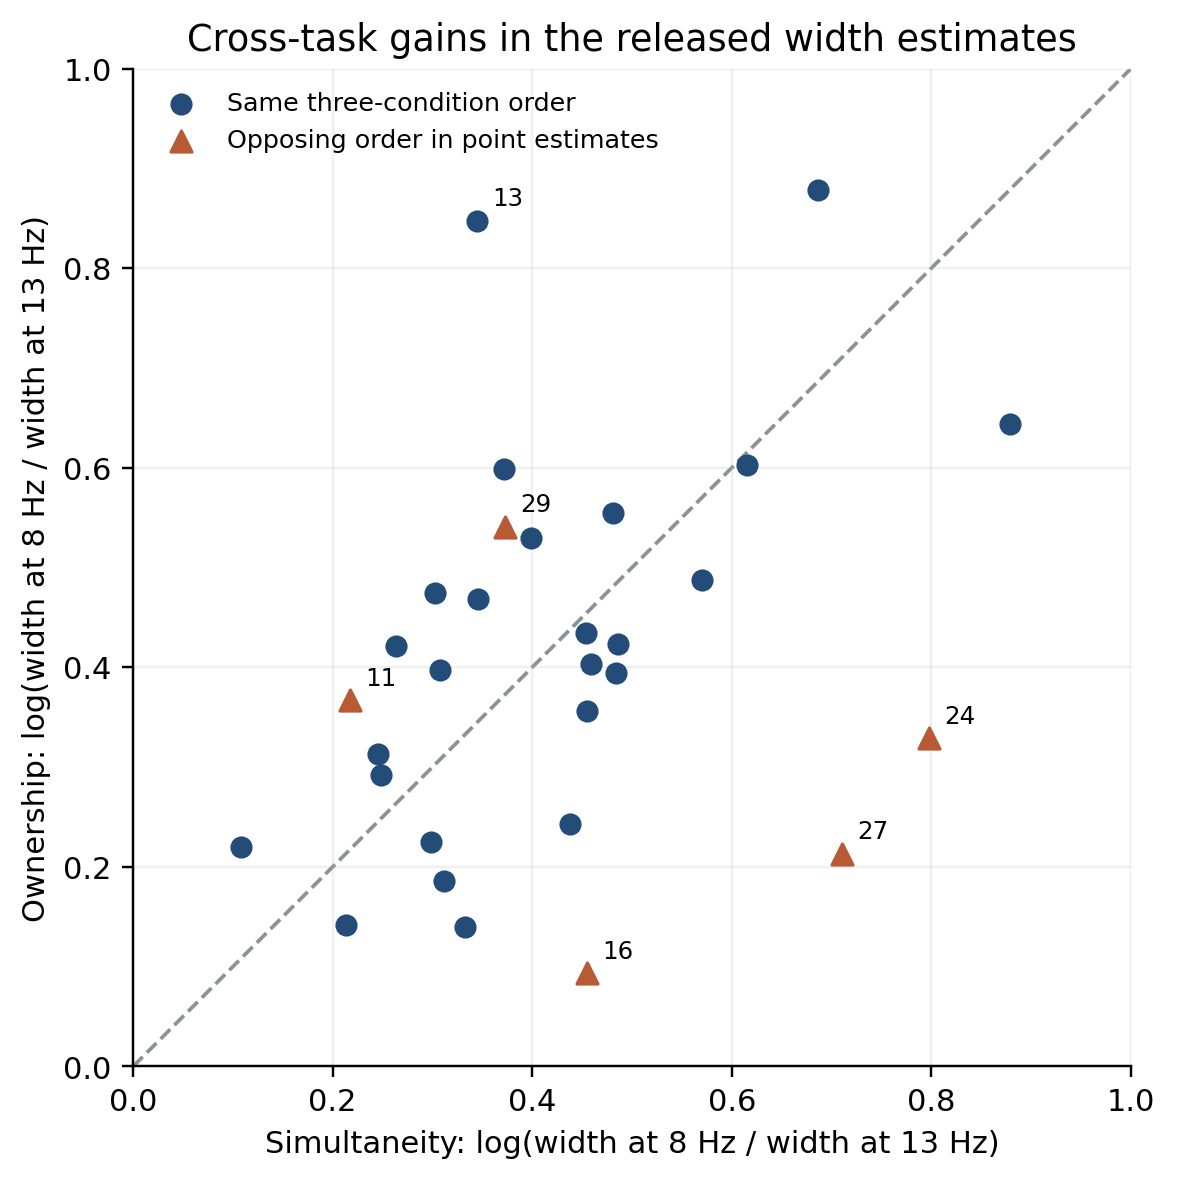
\includegraphics[width=0.75\textwidth,height=\textheight]{../figures/figure1_log_gains.png}
\caption{Participant-level log gains calculated from the 180 released
width estimates. Each point is one participant; the diagonal denotes
equal 8-Hz/13-Hz log gains. Separation from the diagonal is a
fitted-estimate contrast, not a calibrated individual violation.}
\end{figure}

\hypertarget{individual-model-distances-expose-a-different-question}{%
\subsection{5.2 Individual model distances expose a different
question}\label{individual-model-distances-expose-a-different-question}}

The median proportional adjustment budget was
\(\varepsilon_\times^*=0.04112\) log units, corresponding to an upper
multiplicative allowance of 4.20\%. The interquartile range of that
percentage was 1.91\%--6.05\%, and the largest value was 13.39\%. Under
an illustrative 10\% per-cell allowance, 27 of the 30 released matrices
admit a proportional correction.

These are exact descriptive properties of the supplied estimates. A
4.20\% median allowance is neither a measured 4.20\% neural discrepancy
nor evidence that a 4.20\% discrepancy is negligible. It states how much
adjustment is mathematically sufficient and necessary under the chosen
uniform log metric.

Twenty-five participants had exactly the same stimulation ranking across
the two released task profiles. For those point estimates the ordinal
distance is zero, despite possible nonzero proportional distance. Five
had an opposing condition ordering. Without a jointly calibrated error
model for the released estimator, these five are not declared true
violations of a monotone shared scalar. The contrast between the
distances nevertheless makes the assumption hierarchy visible: equal
ratios impose a stronger restriction than compatible order.

\begin{figure}
\centering
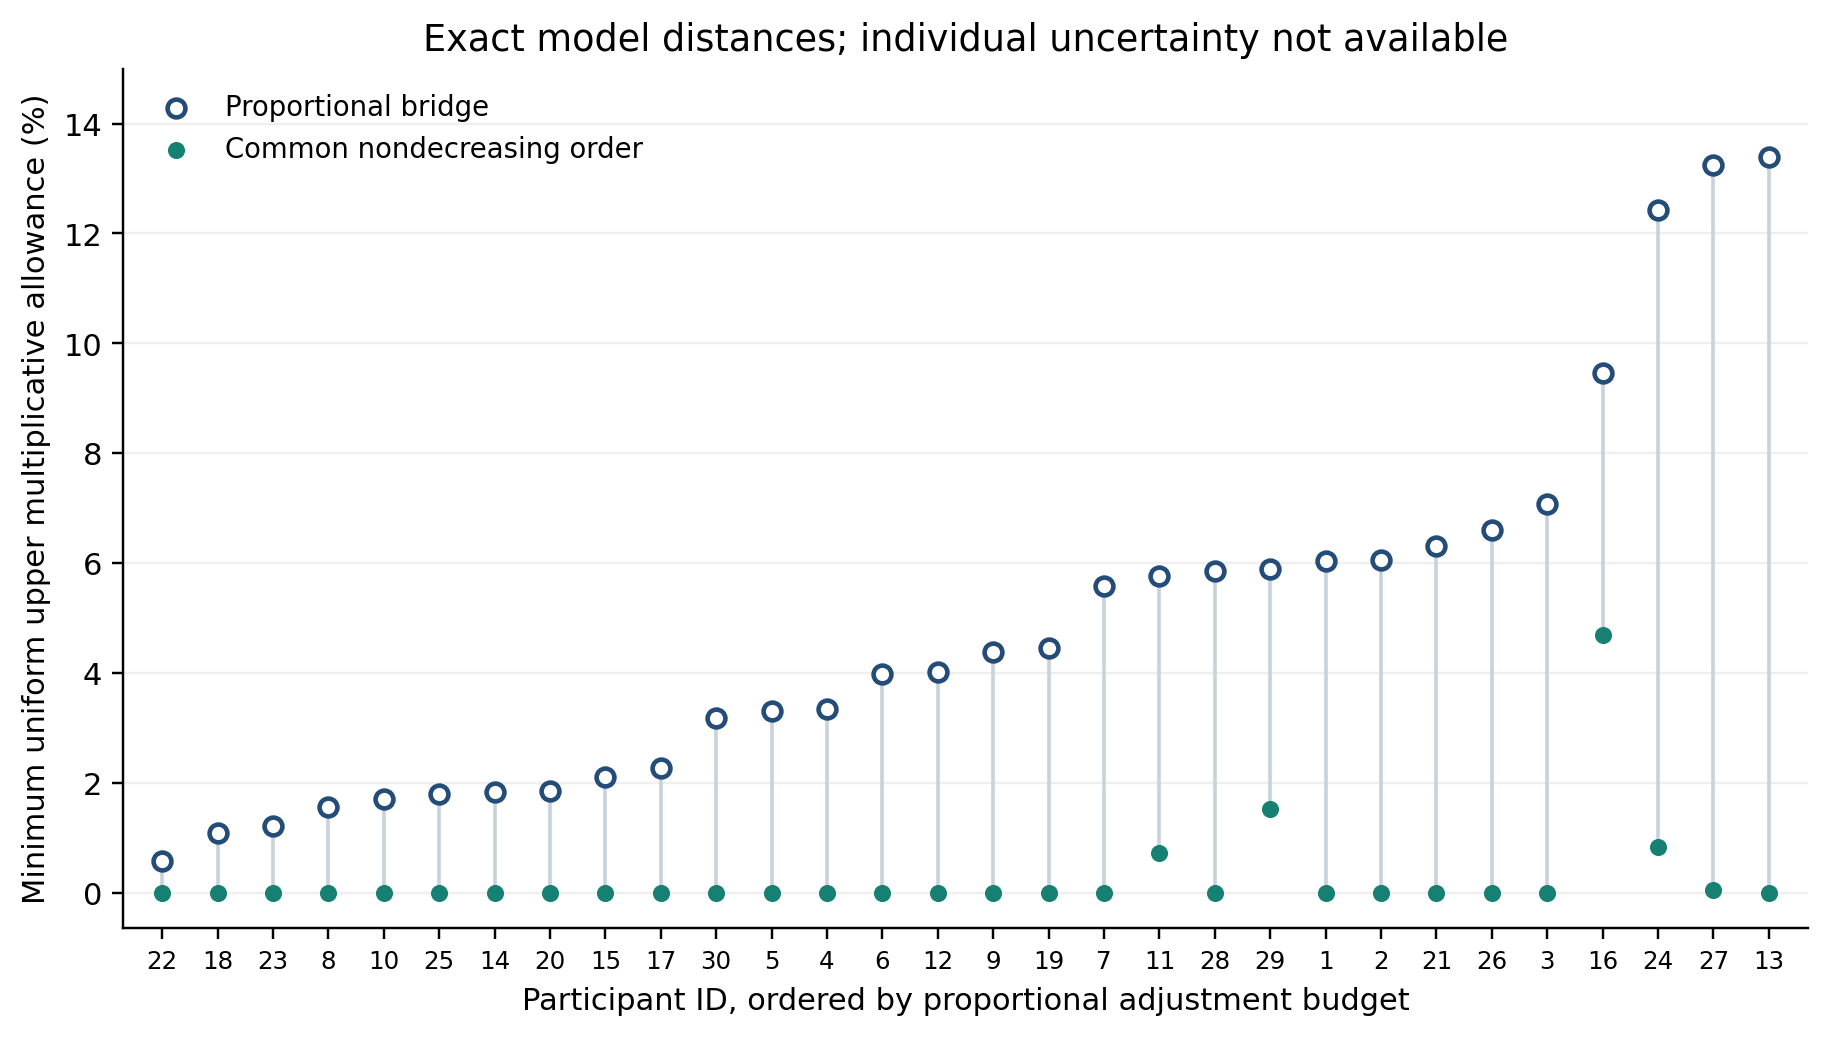
\includegraphics[width=0.95\textwidth,height=\textheight]{../figures/figure2_model_distances.png}
\caption{Exact point-estimate adjustment budgets for both model classes.
Participants are ordered by the proportional budget. The ordinal budget
cannot exceed the proportional budget. Zero ordinal distance means
compatibility with the nondecreasing closure; it does not identify a
physical mechanism.}
\end{figure}

\hypertarget{the-count-likelihood-tests-the-full-set-of-restrictions}{%
\subsection{5.3 The count likelihood tests the full set of
restrictions}\label{the-count-likelihood-tests-the-full-set-of-restrictions}}

For the independently specified binomial Gaussian model, the
unrestricted and restricted negative log likelihoods were 4633.20782 and
4670.11455. The likelihood-ratio statistic was 73.81345 for the 60
proportional restrictions. The descriptive \(\chi^2_{60}\) reference
gives \(p=.10837\). All original participant fits reported convergence.

The 199-replicate parametric bootstrap yielded 20 statistics at least as
large as the observed statistic. The plus-one tail estimate was
\(p=(20+1)/(199+1)=.105\). The 95\% exact binomial interval for Monte
Carlo uncertainty in the simulated tail probability was
\([.06248,.15095]\). This interval concerns finite simulation error, not
uncertainty about the model assumptions. All 5,970 bootstrap participant
fit pairs reported convergence after ten targeted numerical retries. The
restricted and unrestricted fits frequently reached the amplitude upper
bound (29 and 30 participants, respectively), supporting the use of the
explicitly conditional bootstrap rather than treating the chi-square
reference as an exact calibration. The proportional restriction was not
rejected at the conventional .05 level under this specified model.

The unrestricted fit's deviance relative to independent saturated count
cells was 696.21300. A nominal 720-degree-of-freedom reference gives
\(p=.73114\), but sparse cell sizes, boundary behavior, and ignored
dependence limit this diagnostic. A nonsignificant deviance is not proof
that the response shape or latent interpretation is correct.

This analysis addresses a stronger question than a zero average
8-Hz/13-Hz contrast: all 60 within-person proportional restrictions are
tested jointly within the stated count model. Its widths are estimates
under a separately specified fit and are not assumed interchangeable
with the source's released estimates. Neither analysis establishes the
physical number of mechanisms, and agreement in their general direction
is not an independent replication because both derive from the same
study.

\hypertarget{reproducibility-boundary}{%
\subsection{5.4 Reproducibility
boundary}\label{reproducibility-boundary}}

The source's six-column width table and four publisher source-data
blocks were exactly cross-checked. The inherited cross-task intervention
correlations were reproduced. The extraction is therefore traceable. The
attempted least-squares width reconstruction remains incomplete and is
included as a diagnostic, with its fitting choices and examples. No
participant matching algorithm was used to relabel people or repair the
source.

The unresolved reconstruction prevents attaching trial-derived
confidence intervals to the released parameter-level distances. It does
not prevent reproducing the stated arithmetic on those released values
or fitting an independently declared model to the count cells. The
distinction is carried through the code, tables, figures, and claim
ledger.

\hypertarget{what-the-experiment-can-distinguish}{%
\section{6. What the experiment can
distinguish}\label{what-the-experiment-can-distinguish}}

\hypertarget{model-conjunctions-not-theory-names}{%
\subsection{6.1 Model conjunctions, not theory
names}\label{model-conjunctions-not-theory-names}}

The proper unit of a discriminating prediction is a concrete theory
instance together with an intervention model, parameter restrictions,
and a measurement bridge. A broad label such as predictive processing or
UCT does not supply all of these. Table 2 records what is tested here.

\Needspace{29\baselineskip}

\begin{longtable}[]{@{}
  >{\raggedright\arraybackslash}p{(\columnwidth - 4\tabcolsep) * \real{0.3333}}
  >{\raggedright\arraybackslash}p{(\columnwidth - 4\tabcolsep) * \real{0.3333}}
  >{\raggedright\arraybackslash}p{(\columnwidth - 4\tabcolsep) * \real{0.3333}}@{}}
\toprule\noalign{}
\begin{minipage}[b]{\linewidth}\raggedright
Specified account
\end{minipage} & \begin{minipage}[b]{\linewidth}\raggedright
Observable restriction
\end{minipage} & \begin{minipage}[b]{\linewidth}\raggedright
Status in this analysis
\end{minipage} \\
\midrule\noalign{}
\endhead
\bottomrule\noalign{}
\endlastfoot
Multiplicative width bridge & Equal within-person ratios across
conditions & Tested under specified estimators; not established \\
Scalar with stable increasing maps & Same order and matching strict ties
& Descriptive distances; individual uncertainty missing \\
Scalar with condition-specific maps & No cross-condition restriction &
Not discriminable from widths alone \\
Original Bayesian uncertainty model & Its own nonlinear response
predictions & Original comparison inherited; not retested here \\
UCT C1 without an endpoint bridge & No signed numerical width prediction
& Not selected by these data \\
IIT, GNWT, or HOT as broad families & No task-specific prediction
supplied here & Not tested \\
\end{longtable}

\textbf{Table 2.} A scope comparison. A failure of the proportional
bridge would not automatically count against all common-scalar models,
the original Bayesian account, or an entire consciousness theory. A
successful fit would likewise not select one of them.

Experimental theory comparison can be more informative when proponents
agree in advance on divergent predictions and their observation rules.
The Cogitate collaboration illustrates the value and difficulty of such
explicit commitments in consciousness research {[}12{]}. The present
analysis adopts the requirement for explicit commitments; it does not
import that study's predictions into body ownership or assert a
comparable adjudication of global theories.

\hypertarget{uct-interpretation}{%
\subsection{6.2 UCT interpretation}\label{uct-interpretation}}

UCT C1 identifies an admitted actual process token's complete physical
organization with its experiential organization, while distinguishing
that complete object from finite views and estimates {[}10{]}. Its
universal-experience commitment does not make basic experience
conditional on prediction, report, bodily ownership, intelligence, or
the success of a width-model test. Those commitments remain axiomatic in
this paper.

The present measurements are finite task outcomes. Neither the 180
widths nor a fitted latent scale determine complete physical
organization. Even an independently identified neural route would still
require an appropriately justified bridge to a particular experiential
endpoint. Agency, ownership, tactile sensitivity, and familiar mineness
must not be silently substituted for one another; empirical work already
distinguishes aspects of these bodily judgments {[}13,14{]}.

For UCT, the methodological advance is a way to state an additional
bridge sharply enough to fail. It does not establish C1, infer a unique
subject from a statistical factor, or exclude nested and overlapping
actual processes. A common temporal coordinate across tasks also does
not imply that their experiences are identical. Distinct experiential
structures can share an organizational feature.

This separation prevents a tempting but invalid inference: a brain
perturbation changes an ownership report, therefore a specified internal
consumer has been identified, therefore UCT is confirmed. Each
implication requires its own evidence. The source experiment supports
important claims under its own design; the secondary analysis supplies a
narrower test of a new operational restriction.

\hypertarget{why-the-result-remains-useful-without-a-theoretical-winner}{%
\subsection{6.3 Why the result remains useful without a theoretical
winner}\label{why-the-result-remains-useful-without-a-theoretical-winner}}

The data do not compel rejection of the specified proportional response
model. The appropriate response is to retain the result and identify
what was actually constrained. An uninformative generic claim has been
replaced by exact testable equalities, explicit alternatives,
descriptive lower bounds on model adjustment, and a count-level
likelihood test.

The two distances also prevent the wrong follow-up experiment. If only
proportionality fails, the next comparison should address nonlinear or
unstable task bridges before asserting two separate neural processes. If
common order fails beyond defensible uncertainty, the experiment must
distinguish task-map drift, a second latent influence, and
endpoint-model misspecification. Repeating a group-mean contrast cannot
answer those questions.

\hypertarget{a-concrete-prospective-extension}{%
\section{7. A concrete prospective
extension}\label{a-concrete-prospective-extension}}

The original source-consumer question remains physically stronger than
the present dataset: keep selected action and prediction outputs matched
while changing which information reaches a verified consumer, then test
an independently specified experiential endpoint. No such selective
motor-command/proprioceptive intervention was performed in this
reanalysis. The following extension specifies the missing work without
presenting it as an obtained result.

First, define one actual installation and a limited target: for example,
an identified sensorimotor prediction consumer and a separately
calibrated ownership or agency judgment. Source identities, consumer
ports, timing, task instructions, learning state, and the scope of
output matching must be recorded. Equality of a selected action
trajectory does not establish equality of all afferent information.
Conversely, a decoding signal at a region does not establish consumption
by the downstream process.

Second, specify competing models before selecting diagnostic
interventions. A fixed match-only account predicts equal endpoint
distributions whenever its selected prediction-error input and response
mapping are matched. A route-sensitive account must name an additional
consumer relation and state a distinct, signed or quantitatively bounded
prediction for the same endpoint. A broad forward-model or UCT label is
insufficient. Prior agency models already show why a match-only account
is an especially restricted comparator {[}15,16{]}. It should not stand
in for all existing theories.

Third, use separate calibration data to constrain each measurement
bridge, then freeze it for held-out interventions. A task factor or
monotone map estimated anew in every condition can absorb the sought
discrepancy. Use repeated measurements and record trial/block order so
the joint uncertainty can be propagated through the actual estimator.
The interval corollary gives a concrete decision rule when simultaneous
log-width bounds are warranted: an independently justified error
rectangle must remain separated from the tested model class. Other
endpoints require their own corresponding rule.

Fourth, validate intervention selectivity and the actual consumer
relation. A source block that also changes a direct pathway can mimic
mediation. An apparent rescue can instead be compensation by a newly
learned reader. Prior source-consumer work makes these distinctions
explicit {[}2{]}; the prospective experiment must establish the relevant
exclusion and timing assumptions, rather than infer them from endpoint
recovery alone.

Finally, report outcomes at the level their premises support. A held-out
discrepancy beyond both estimation error and allowed bridge drift can
reject a specified model conjunction. The result becomes comparative
evidence between theories only when their alternative, faithful model
instances predict distinguishable observations under the same validated
intervention. An unchanged endpoint may reflect a shared feature,
compensation, insufficient precision, or an insensitive bridge. It
cannot establish absence of experience.

This is a prospective design contract, not a power calculation or an
approved human protocol. The present aggregate data do not provide the
estimator reliability, trial dependence, or scientifically motivated
minimum separation needed to justify a new participant number. Those
quantities must be estimated in an appropriate pilot or recovered from
the original analysis pipeline before prospective recruitment.

\hypertarget{limitations-and-contribution-statement}{%
\section{8. Limitations and contribution
statement}\label{limitations-and-contribution-statement}}

The mathematical results are applications of classical rank-one,
Chebyshev, and isotonic principles. The study does not claim a new
branch of mathematics, the first common-latent-order test, or the first
neural intervention on bodily perception. The internal and external
novelty search found no previous report of this exact proportional-width
reanalysis in the checked materials, but cannot establish universal
priority.

The empirical contribution is restricted to one selected 30-person
dataset, released fitted parameters, and an independently specified
response model. The analyses are retrospective, share the same source
observations, and have no independent replication. The source sample's
illusion susceptibility, the absence of trial-order records, the
unresolved source-estimator reconstruction, and the arbitrary
illustrative equivalence margins limit inference.

The selected endpoints are judgments and fitted response
characteristics. Their relation to sensory uncertainty, neural timing,
ownership experience, or familiar self-related experience requires
additional validation. The intervention effect does not alone identify a
mediator or a particular information-consumer route. UCT C1 remains an
inherited interpretive axiom; global consciousness theories were not
adjudicated.

The defensible originality statement is therefore: \textbf{we formulate
and retrospectively test a specific cross-task proportional-width
constraint, report exact distances to both proportional and ordinal
model classes, and use the resulting evidence to state which
mechanism-to-endpoint inferences remain unlicensed.} This is a methods
and secondary-analysis contribution. The prospective scientific advance
will require independently calibrated bridges and a physically validated
intervention that generates genuinely divergent held-out predictions.

\hypertarget{reproducibility-data-rights-and-disclosures}{%
\section{Reproducibility, data rights, and
disclosures}\label{reproducibility-data-rights-and-disclosures}}

The accompanying package contains unchanged public input files,
provenance and checksum records, the extraction and analysis code,
per-participant tables, independent mathematical checks, fitting
diagnostics, figures, a claim-level originality audit, and a Chinese
research handoff. The original article and publisher source data are
attributed to D'Angelo et al.~{[}1{]} under the source's stated terms;
original files are not relabeled as newly collected data. The package
records observed rights information and separates new code from
third-party materials.

Computations use Python, NumPy, SciPy, pandas, and openpyxl; figures use
Matplotlib. Exact versions, random seeds, numerical bounds, fit
statuses, and reproduction commands are included. The deterministic
width contrasts and mathematical checks can be rerun independently of
the longer count bootstrap. Finite checks are not human data;
parametric-bootstrap samples are explicitly simulated conditional
datasets.

Substantial ChatGPT (OpenAI GPT-6 Astra Pro) assistance was used for
retrieval, analysis, derivation, internal adversarial review, drafting,
and preparation under human direction. Collaborating AI passes are not
independent human peer review. No final human line-by-line verification
or external scientific endorsement is claimed. The author of record is
responsible for deciding whether and how to release a later public
edition. No correspondence with source authors was sent as part of this
analysis.

\hypertarget{references}{%
\section{References}\label{references}}

\begin{enumerate}
\def\labelenumi{\arabic{enumi}.}
\item
  D'Angelo, M., Lanfranco, R. C., Chancel, M., \& Ehrsson, H. H. (2026).
  Parietal alpha frequency shapes own-body perception by modulating the
  temporal integration of bodily signals. \emph{Nature Communications,
  17}, 53.
  \href{https://doi.org/10.1038/s41467-025-67657-w}{doi:10.1038/s41467-025-67657-w}.
  Public data: \href{https://osf.io/ytga5/}{osf.io/ytga5}; modeling
  code: \href{https://osf.io/s5p4v/}{osf.io/s5p4v}.
\item
  Liu, H. (2026). \emph{Matched Behavior and Source Use: Exact
  intervention protocols, consumer classes, and limits of sensorimotor
  interpretation} (SCU-PAPER-v1.0.1). Theoretical and computational
  preprint.
  \href{https://doi.org/10.5281/zenodo.23272690}{doi:10.5281/zenodo.23272690}.
\item
  Bamber, D. (1979). State-trace analysis: A method of testing simple
  theories of causation. \emph{Journal of Mathematical Psychology, 19},
  137--181.
  \href{https://doi.org/10.1016/0022-2496(79)90016-6}{doi:10.1016/0022-2496(79)90016-6}.
\item
  Prince, M., Brown, S., \& Heathcote, A. (2012). The design and
  analysis of state-trace experiments. \emph{Psychological Methods, 17},
  78--99. \href{https://doi.org/10.1037/a0025809}{doi:10.1037/a0025809}.
\item
  Kalish, M. L., Dunn, J. C., Burdakov, O. P., \& Sysoev, O. (2016). A
  statistical test of the equality of latent orders. \emph{Journal of
  Mathematical Psychology, 70}, 1--11.
  \href{https://doi.org/10.1016/j.jmp.2015.10.004}{doi:10.1016/j.jmp.2015.10.004}.
\item
  Stout, Q. F. (2015; revised 2017). \emph{L infinity isotonic
  regression for linear, multidimensional, and tree orders}.
  \href{https://arxiv.org/abs/1507.02226}{arXiv:1507.02226}.
\item
  Yarrow, K., Solomon, J. A., Arnold, D. H., \& Roseboom, W. (2023). The
  best fitting of three contemporary observer models reveals how
  participants' strategy influences the window of subjective synchrony.
  \emph{Journal of Experimental Psychology: Human Perception and
  Performance, 49}, 1534--1563.
  \href{https://doi.org/10.1037/xhp0001154}{doi:10.1037/xhp0001154}.
\item
  Luce, R. D., \& Tukey, J. W. (1964). Simultaneous conjoint
  measurement: A new type of fundamental measurement. \emph{Journal of
  Mathematical Psychology, 1}, 1--27.
  \href{https://doi.org/10.1016/0022-2496(64)90015-X}{doi:10.1016/0022-2496(64)90015-X}.
\item
  Loftus, G. R. (1978). On interpretation of interactions. \emph{Memory
  \& Cognition, 6}, 312--319.
  \href{https://doi.org/10.3758/BF03197461}{doi:10.3758/BF03197461}.
\item
  Liu, H. (2026). \emph{Unified Consciousness Theory I:
  Structural--Experiential Identity and the Continuity from Physical
  Process to Conceptual Self} (v1.2). Theoretical preprint.
  \href{https://doi.org/10.5281/zenodo.23131575}{doi:10.5281/zenodo.23131575}.
\item
  Liu, H. (2026). \emph{Unified Consciousness Theory II: Consciousness
  Theories as Effective Organization Theories} (v1.1). Theoretical
  preprint.
  \href{https://doi.org/10.5281/zenodo.23030320}{doi:10.5281/zenodo.23030320}.
\item
  Cogitate Consortium et al.~(2025). Adversarial testing of global
  neuronal workspace and integrated information theories of
  consciousness. \emph{Nature, 642}, 133--142.
  \href{https://doi.org/10.1038/s41586-025-08888-1}{doi:10.1038/s41586-025-08888-1}.
\item
  Kalckert, A., \& Ehrsson, H. H. (2012). Moving a rubber hand that
  feels like your own: A dissociation of ownership and agency.
  \emph{Frontiers in Human Neuroscience, 6}, 40.
  \href{https://doi.org/10.3389/fnhum.2012.00040}{doi:10.3389/fnhum.2012.00040}.
\item
  Liu, H. (2026). \emph{Experience, Intelligence, and Self Within
  Experience: Definitions, Conditional Theorems, and Thought Experiments
  for a Structural Account} (v1.0). Theoretical preprint.
  \href{https://doi.org/10.5281/zenodo.23206492}{doi:10.5281/zenodo.23206492}.
\item
  Zaadnoordijk, L., Besold, T. R., \& Hunnius, S. (2019). A match does
  not make a sense: On the sufficiency of the comparator model for
  explaining the sense of agency. \emph{Neuroscience of Consciousness,
  2019}, niz006.
  \href{https://doi.org/10.1093/nc/niz006}{doi:10.1093/nc/niz006}.
\item
  Legaspi, R., \& Toyoizumi, T. (2019). A Bayesian psychophysics model
  of sense of agency. \emph{Nature Communications, 10}, 4250.
  \href{https://doi.org/10.1038/s41467-019-12170-0}{doi:10.1038/s41467-019-12170-0}.
\item
  Dunn, J. C., \& Anderson, L. M. (2026; first published online 2024).
  The monotonic linear model: Testing for removable interactions.
  \emph{Psychological Methods, 31}, 585--606.
  \href{https://doi.org/10.1037/met0000626}{doi:10.1037/met0000626}.
  This is additional close prior art for monotonicity-based interaction
  tests; no priority over that established program is claimed.
\end{enumerate}

\end{document}
